
% latex-sample.tex
%
% This LaTeX source file provides a template for a typical research paper.
%

%
% Use the standard article template.
%
\documentclass[12pt, a4paper, twocolumn]{article}

% The geometry package allows for easy page formatting.
\usepackage{geometry}
\usepackage{multicol}
\usepackage{float}
\geometry{letterpaper}

% Load up special logo commands.
\usepackage{doc}

% Package for formatting URLs.
\usepackage{url}

% Packages and definitions for graphics files.
\usepackage{graphicx}
\usepackage{epstopdf}
\title{DBCheck: Model-Based Concurrency Verification}
\author{Charles Dake}
\date{}

%
% Set the title, author, and date.
%

%
% The document proper.
%
\begin{document}

% Add the title section.

% Add an abstract.


\maketitle
\abstract{
A critical area of DBMS systems is the concurrency model. DBMS systems often handle large volumes of transactions in short intervals. Concurrency models are key here in handling such volumes. Concurrency also exposes the DBMS system to vulnerabilities to its durability and integrity. One point of vulnerability is the effect of the scheduling of operations and transactions on database integrity. The author in this paper explores how model checking may be used as a technology to verify the design assumptions in database concurrency model design. Two Phase Locking (2PL) will be used as an existing standard to compare results.}



% Body text.
%
\section{Introduction}
\label{introduction}
In the design and operation of DBMS systems, enforcing the ACID properties of the system is of critical importance \cite{textbook}. This in turn implies the importance of having effective methods to test and measure a system's observance of ACID properties. Formal methods are one approach to building systems with secure designs. Model checking is an example of a formal method with the capacity to test design concepts. 

Temporal Logic Model Checking is a one variant with major application in verification and validation of both software and hardware systems. Examples of successful verification of industrial systems include the PCI Local Bus, an aircraft controller and a medical monitoring system \cite{McMillian1993}. In particular, these examples have made used of the Symbolic Model Verifier (SMV). The technology used in this application is NuSMV, which is a variant based off of SMV. These technologies use temporal model checking, which is one form of model checking where there exists efficient algorithms.

In temporal logic model checking, the model checker accepts a model specification and specifications written in temporal logic. It in turn checks the validity of these specifications and furnishes counter examples if there are any. Due to the capacity for temporal logic to express propertiecs involving timing conditions, concurency systems are a natural domain for this form of model checking \cite{temporal}.



\section{Database Concurrency}
In Database Design, one major assumption is the database’s ACID properties (atomic, consistency, isolation, durability). The database model’s concurrency is one source of problems for these properties. An improperly implemented concurrency model can create inconsistent database states, make the database inoperable with problems such as deadlock, and corrupt the database in the instance of failure. Concurrency models can be improved by making sure the execution of database transactions is serializable. This ensures that transactions which are executed concurrently have a serializable schedule such that their effect won’t differ from a non-concurrent order of execution.



\section{2PL}
2PL or two phase locking is one standard used to ensure serializability. 2PL, as the name implies, involves the use of two lock phases for processes.

\begin{enumerate}
\item Growing Phase: The process obtains all its locks and does not release any.
\item Shrinking Phase: The process releases all its locks and does not obtain any new ones.
\end{enumerate}

2PL is stated to guarantee serializability. There are a number of variations of 2pl, with the most widely used being Strict 2PL \cite{textbook}. According to \cite{textbook}, Strict 2PL has two rules 
“If a transaction T wants to read (respectively, modify an object, it first requests a shared (respectively, exclusive) lock on the object.”
“ All locks held by a transaction are released when the transaction is completed.”
In practice, an architect of a DBMS (database management system) using this protocol may expect that the serializable property will hold. In the rest of the work, the testing of this property and others will be explored. A precise formal analysis of the properties of the protocol will not be taken. The protocol instead will be tested with respect to a computational model for concurrent execution which has been defined by the author.



\section{NuSMV}
The technology used in the model checking analysis is the NuSMV symbolic model checker. NuSMV works by defining the model of a state machine. This is in effect a transition system with a number of states and rules which determine the transitioning between states. NuSMV allows for the definition of objects or modules with basic data structures and operations. The model checking of these model workings by testing specifications against the models to determine the truth or falsity of the specifications for the models. The specification languages used are LTL (Linear Temporal Logic) and CTL (Computational Tree Logic). For the purposes of the author, only CTL was required.

\section{CTL}
CTL or Computational Temporal Logic is a variant of temporal logic which explores the truth of states in regard to the future paths from  a given state. In NuSMV, this would be the initial state of the model. The language itself consists of a number of quantifiers and atomic propositions.
\begin{enumerate}
\item EG - Exists Globally
\item EX - exists Next
\item EF - exists finally
\item AG - For all Globally
\item AX - for all next
\item AF - for all finally
\end{enumerate}
The atomic propositions in NuSMV will correspond to the values of the variables  and module which make up the model.


\section{DBCheck}
The author’s model checking project was named NuSMV. The models used in this work are all variations of a general concurrency model. This model consists of a process module and memory cell module. At this point, all the models are implemented with 2 processes and 2 memory cells. 


\begin{figure}[H]
	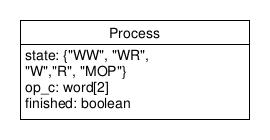
\includegraphics[width=\linewidth]{dbcheck_model.jpg}
\end{figure}

This intent of the process module is to represent the action of a database transaction thread. For the purposes of this work, the memory cell only implements the lock for a given database resource. Depending on the variations of the model’s implementation, the internal logic will differ and some execute with respect to different input or internal parameters.

\subsection{DBCheck Models}
For the testing purposes, DBCheck currently has 4 main model classes. These are a Strict 2PL model, a Conservative 2PL model, a naive model, and a final additional model, C1. Each of the models has 2 versions, a 2 operation schedule version and a 4 operation schedule version. 

\subsection{DBCheck Specs}
DBCheck Specs
In testing the model’s adherence to the serializability property or other properties of an ACID DBMS, different levels of rigor may be used as to the result. Also, the generality of the model allows for different granularities. In a practical implementation,  the specifications may involve the literal semantics of the data. In the testing at this stage of DBCheck, the specifications are situated around three different possible forms of occurrence in a non-serializable model. These are WW errors, WR errors and RW errors. A stated problem with Strict 2PL is that it may have issues with deadlock. For this reason, a deadlock specification is also used. The specifications are shown with their CTL syntax.
\begin{enumerate}
\item $AG ((p1.state[i] = “W”)  \implies (AG \neg( \negP1.finished \land p2.state[i]=”W”))$
This says that in the model that if a process p1 has a write operation on resource i, then in every following state it cannot be true that p1 has not finished and p2 has a write operation on resource i. This would correspond to a blind write. 
\item $AG ((p1.state[i] = “R”)  \implies (AG \neg(\neg P1.finished \land p2.state[i]=”W”))$
This says that in the model that if a process p1 has a read operation on resource i, then in every following state it cannot be true that p1 has not finished and p2 has a write operation on resource i.
\item $AG ((p1.state[i] = “W”)  \implies (AG \neg(\neg P1.finished \land p2.state[i]=”R”))$
This says that in the model that if a process p1 has a write operation on resource i, then in every following state it cannot be true that p1 has not finished and p2 has a read operation on resource i.
\end{enumerate}

These properties are all expected to hold within 2PL. This should be true with respect to both Strict 2PL and Conservative 2PL. However, their implication to serializability rests on order assumptions. DBCheck does not have a serializable order defined for all models. For the naive model and strict 2PL there is no order defined for the model. In C1 and C2PL, the models do have an order defined.  The two final properties are a property for 2PL and the deadlock property. 

\begin{enumerate}
	\item $AF (p1.finished \land p2.finished)$

	This property just asserted that the schedules always finish. Later in the results, an example is shown of a conuterexample to this specification for Strict 2PL which shows a deadlock situation.

	\item $G (( acell.lock = 1 \land X ( acell.lock = 0)) \implies X(G \neg (acell.lock = 1)))$

		This property, which is actually defined separety for the model based on the lock definition, expresses that for each process, if it has released a lock it doesn't reqaquire it.

\end{enumerate}

This is defined loosely as 
AF ( p1.finished \& p2.finished)
The meaning of this is that in all states there exists a future state where both processes have finished.



\section{Testing}
These properties are all expected to hold within 2PL. This should be true with respect to both Strict 2PL and Conservative 2PL. However, their implication to serializability rests on order assumptions. DBCheck does not have a serializable order defined for all models. For the naive model and strict 2PL there is no order defined for the model. In C1 and C2PL, the models do have an order defined.  The final property is the deadlock property. This is defined loosely as 
AF ( p1.finished \& p2.finished)
The meaning of this is that in all states there exists a future state where both processes have finished.


\begin{tabular}{l||llll}
&Deadlock&WW&WR&RW\\\hline
Simple 2op&64/256&216/256&216/256&144/256\\
S2PL 2op&256/256&256/256&256/256&256/250\\
C2PL 2op&256/256&256/256&256/256&256/250\\
Naive 4op&<++>/65536&<++>/65536&<++>/65536&<++>/65536\\
S2PL 4op&<++>/65536&<++>/65536&<++>/65536&<++>/65536\\
C2PL 4op&65536/65536&65536/65536&65536/65536&65536/65536\\
\end{tabular}


From the results above, the stated behavior of strict 2pl and c2pl can be observed. Strict 2pl succeeds on all the serialzability specifications but does not on the deadlock specification. Conservative 2pl succeeds on all specifications. As expected a simple lock does not meet the serializability criterion. 

\section{Samples}
\subsection{S2PL Deadlock}
Shown below is an example of the S2PL lock in deadlock. This example is pulled from a counterexample generated in testing the deadlock specification on a S2PL configuration.

\begin{figure}[H]
	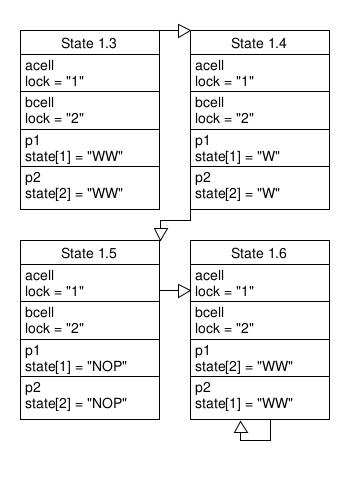
\includegraphics[width=\linewidth]{2pl_deadlock.jpg}
\end{figure}

\subsection{Simple Lock WW Failure}
This figure shows the state diagram of a counterexample for the WW serializability spec. The simple lock is not designed for schedule serializability. The figure shows an example of the specification not holding for the model.

\begin{figure}[H]
	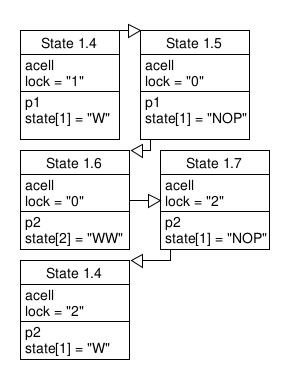
\includegraphics[width=\linewidth]{simple_WW.jpg}
\end{figure}

\section{Conclusion}
The results of DBCheck show the potential of this form of Model Checking in a tool for model validation. The stated properties of the 2PL protocols variants are correspondingly observed in the results of the specification testing. The results, however, speak for the model tested and the 2PL protocols themselves. Further efforts could be underdone to formalize the protocol standard and then find a representative model from which general results. A verfication fo the Kerberos protocol is done with NuSMV by M. Panti L. Spalazzi and S. Tacconi \cite{kerberos}. 

Since the 2PL standards themselves follow a loose system of definition, another application is in the validation of the implementation model of the protocol. From this vantage, the models instead are supposed to represent specific architectures using the 2PL standard. In the DBCheck implementation, the models are abstract and miniature in scale. Since the validation of the model corresponds only so far as the model represents the behavior of the system, a further objective here is creating models that better represent the system behavior. With more exhaustive model definition, the opportunites for the verification of ACID properties such as durability also will open up. For example, this could be seen in the DBCheck models if the models also accounted for occurences such as abort sequences and system failures.

One barrier to the use of model checking are the complexity challenges involved. An example of this is seen in DBCheck as the number of possible schedules. For the models in use, the runtime of any model with a specific schedule is minimal (seconds or less). The problem arrises however in the combinatorics of the possible schedules that the system may encounter. This value is exponentially correlated to the number of operations in a schedule. As a result, the model checking may prove infeasible with schedules of arbitrary size. 

In conclusion, the applicability of NuSMV for the verification purposes of both implemented system and protocol is clearly apperent. The use of model checking for both purposes is the site of substantial application. Further research in the database concurrency and transaction management could involve more rigorous specfication of ACID properties within the domain of temporal logic. The computational models of database system could be further defined for the comparison of results. A potential outcome of this research would be a the design of an tool and accompanying engineering testing methodology for the specfication and testing of DBMS systems.


\bibliographystyle{plain}
\bibliography{dbcheck}

\end{document}
